\newpage
\section{Resultados e discussão}

% =============== EXPERIMENTO 1 ===================== %

\subsection{Determinação do Momento de Inércia de um disco}

Baseado no vídeo disponibilizado, logo abaixo temos uma tabela que reuni os valores medidos experimentalmente e que utilizaremos nos nossos cálculos para determinar I fisicamente:

\begin{table}[H]
    \centering
    \begin{tabular}{ |p{5cm}||p{2cm}||p{2cm}||p{2cm}|  }
        \hline
        \textbf{O que foi medido} & \textbf{Valor} & \textbf{Incerteza} & \textbf{Unidade}\\
        \hline
        Massa do anel (m\textsubscript{a})          & 0,9238    & $\pm$ 0,0001  & kg\\
        Massa do disco (m\textsubscript{d})         & 0,4707    & $\pm$ 0,0001  & kg\\
        Massa do eixo (m\textsubscript{e})          & 0,12125   & $\pm$ 0,00001 & kg\\
        Raio do eixo (R\textsubscript{e})           & 0,0060    & $\pm$ 0,0001  & m\\
        Raio menor do disco (R\textsubscript{d1})   & 0,0060    & $\pm$ 0,0001  & m\\
        Raio maior do disco (R\textsubscript{d})    & 0,0625    & $\pm$ 0,0001  & m\\
        Raio menor do anel (R\textsubscript{a1})    & 0,0625    & $\pm$ 0,0001  & m\\
        Raio maior do anel (R\textsubscript{a})     & 0,0760    & $\pm$ 0,0001  & m\\
        \hline
    \end{tabular}
    \caption{Dimensões e propriedades físicas do Disco de Maxwell}
\end{table}

Utilizado esses valores, podemos calcular os momentos de inércia:

\[I_E = \frac{1}{2} \cdot m_e \cdot R_e^2\]
\[I_E = \frac{1}{2} \cdot 0,12125 \cdot (0,0060)^2 = 0,0000021825 (kg \cdot m^2)\]

\[I_D = \frac{1}{2} \cdot m_d \cdot (R_{d1}^2 + R_d^2)\]
\[I_D = \frac{1}{2} \cdot 0,4707 \cdot [(0,0060)^2 + (0,0625)^2] = 0,0009278085 (kg \cdot m^2) \]

\[I_A = \frac{1}{2} \cdot m_a \cdot (R_{a1}^2 + R_a^2)\]
\[I_A = \frac{1}{2} \cdot 0,9238 \cdot [(0,0625)^2 + (0,0760)^2] = 0.0044722313 (kg \cdot m^2) \]

E consequentemente as incertezas desses valores serão:

\[\Delta I_E = \frac{1}{2} \left( \Delta m_e \cdot R_e^2 + 2 \cdot R_e \cdot \Delta R_e \cdot m_e \right)\]
\[\Delta I_E = \frac{1}{2} \left( 0,00001 \cdot (0,0060)^2 + 2 \cdot 0,0060 \cdot 0,0001 \cdot 0,0001 \right) = 0.000000000078 (kg \cdot m^2)\]

\[\Delta I_D = \frac{1}{2} 
    \left[ 
        \Delta m_d \cdot (R_{d1}^2 + R_d^2) + 
        \left( 2 \cdot R_d \cdot \Delta R_d + 2 \cdot R_{d1} \cdot \Delta R_{d1} \right) \cdot m_d
    \right]
\]
\[\Delta I_D = \frac{1}{2} 
    \left[ 
        0,0001 \cdot ((0,0060)^2 + (0,0625)^2) + 
        \left( 2 \cdot 0,0625 \cdot 0,0001 + 2 \cdot 0,0060 \cdot 0,0001 \right) \cdot 0,4707
    \right]
\]
\[\Delta I_D = 0.0000034214 (kg \cdot m^2)\]

\[\Delta I_A = \frac{1}{2} 
    \left[ 
        \Delta m_a \cdot (R_{a1}^2 + R_a^2) + 
        \left( 2 \cdot R_a \cdot \Delta R_a + 2 \cdot R_{a1} \cdot \Delta R_{a1} \right) \cdot m_a
    \right]
\]
\[\Delta I_A = \frac{1}{2} 
    \left[ 
        0,0001 \cdot ((0,0625)^2 + (0,0760)^2) + 
        \left( 2 \cdot 0,0760 \cdot 0,0001 + 2 \cdot 0,0625 \cdot 0,0001 \right) \cdot 0,9238
    \right]
\]
\[\Delta I_D = 0.0000132787 (kg \cdot m^2)\]

Com os momentos de cada peça, podemos agora somá-los:

\[I_T = I_E + I_D + I_A\]
\[I_T = 0,0000021825 + 0,0009278085 + 0,0044722313 = 0,0054022223 (kg \cdot m^2)\]

\[\Delta I_T = \Delta I_E + \Delta I_A + \Delta I_D\]
\[I_T = 0,000000000078 + 0,0000034214 + 0,0000132787 = 0,000016700178 (kg \cdot m^2)\]

Assim, ajustando os algarismos temos que o momento de inércia da Roda de Maxwell do laboratório vale:

\[\therefore \mathbf{I_T = 0,00540 \pm 0,00002 (kg \cdot m^2)}\]

Uma parte do experimento foi concluída. Agora, vamos determinar indiretamente o valor da incerteza utilizando o método da queda. Os dados obtidos estão na tabela abaixo.

\begin{table}[H]
    \centering
    \begin{tabular}{ |p{6cm}||p{2cm}||p{2cm}||p{2cm}|  }
        \hline
        \textbf{O que foi medido} & \textbf{Valor} & \textbf{Incerteza} & \textbf{Unidade}\\
        \hline
        Altura (h)                                      & 0,467 & $\pm$ 0,001 & m\\
        Tempo de queda inicial 1 (t\textsubscript{1i})  & 0,219 & $\pm$ 0,001 & s\\
        Tempo de queda final 1 (t\textsubscript{1f})    & 0,312 & $\pm$ 0,001 & s\\
        Intervalo 1 (t\textsubscript{1})                & 0,093 & $\pm$ 0,002 & s\\
        Tempo de queda inicial 2 (t\textsubscript{2i})  & 0,219 & $\pm$ 0,001 & s\\
        Tempo de queda final 2 (t\textsubscript{2f})    & 0,311 & $\pm$ 0,001 & s\\
        Intervalo 2 (t\textsubscript{2})                & 0,092 & $\pm$ 0,002 & s\\
        Tempo de queda inicial 3 (t\textsubscript{3i})  & 0,222 & $\pm$ 0,001 & s\\
        Tempo de queda final 3 (t\textsubscript{3f})    & 0,312 & $\pm$ 0,001 & s\\
        Intervalo 3 (t\textsubscript{3})                & 0,090 & $\pm$ 0,002 & s\\
        \hline
    \end{tabular}
    \caption{Dados experimentais da queda do Disco de Maxwell}
\end{table}

Primeiramente vamos determinar o tempo médio de queda utilizando a média aritmética entre os intervalos calculados:

\[\overline{t}_b = \frac{t_{b1} + t_{b2} + t_{b3}}{3} = \frac{0,093 + 0,092 + 0,900}{3} = 0,0916666667 (s)\]

\[\Delta \overline{t}_b = \sqrt{\frac{\sum_{i=1}^{3} (t_i - \overline{t})^2}{3}}\]
\[\Delta \overline{t}_b = \sqrt{\frac{(0,093-0,916666667)^2 + (0,092-0,916666667)^2 + (0,900-0,916666667)^2}{3}}\]
\[\Delta \overline{t}_b = 0.001247219 (s)\]

\[\therefore \overline{t} = 0,092 \pm 0,001 (s)\]

Com o tempo médio, podemos aplicar todos os valores na nossa fórmula do momento para queda do Disco de Maxwell:

\[m = m_a + m_d + m_e = 0,9238 + 0,4707 + 0,12125 = 1,51575 (kg)\]

\[I = \left( \frac{g \overline{t}_b^2}{2h} - 1 \right) m r_e^2\]
\[I = \left( \frac{9,80665 \cdot (0,092)^2}{2 \cdot 0,467} - 1 \right) \cdot 1,51575 \cdot (0,0060)^2\]
\[I = \left(0,91113117 \right) \cdot 0,008754972 = 0,0049718 (kg \cdot m^2)\]

E as incertezas para esses valores calculados acima se dão por:

\[\Delta m = \Delta m_a + \Delta m_d + \Delta m_e = 0,0001 + 0,0001 + 0,00001 = 0,00021 (kg)\]

\[
    \Delta P = \frac{g}{2} 
    \left( 
        \frac
        {\overline{t}_b^2 \cdot \Delta h + 2 \cdot \overline{t}_b \cdot \Delta \overline{t}_b \cdot h}
        {h^2} 
    \right)
\]
\[
    \Delta P = \frac{9,80665}{2} \left(\frac{(0,092)^2 \cdot 0,001 + 2 \cdot 0,092 \cdot 0,001 \cdot 0,467}{(0,467)^2} \right) = 0,002122228
\]
\[\Delta Q = 2mr \Delta r + \Delta m r^2\]
\[\Delta Q = 2 \cdot 1,51575 \cdot 0,0001 + 0,00021 \cdot (0,0060)^2 = 0,00003032256\]

\[\Delta I = \Delta P \cdot Q + \Delta Q \cdot P\]
\[\Delta I = 0,002122228 \cdot 0,008754972 + 0,00003032256 \cdot 0,91113117 = 0,0000462079 (kg \cdot m^2)\]

Finalmente, ajustando os algarismos significativos teremos então:

\[\mathbf{I = 0,00497 \pm 0,00005 (kg \cdot m^2)}\]

- comparar os resultados

% =============== EXPERIMENTO 2 ===================== %

\subsection{Choques Rotacionais}

Conforme descrito na Metodologia, o primeiro dado a ser calculado é o Momento de Inércia da peça 2 conforme sua configuração geométrica e sua massa. Para realizar esse cálculo, utilizaremos a seguinte expressão para corpos cilíndricos ocos:

\[I_{CM} = \frac {1}{2}M(R_1^2+R_2^2)\]

sendo que:\\

\begin{table}[H]
    \centering
    \begin{tabular}{ |p{4.3cm}||p{1.7cm}||p{2cm}||p{2cm}|  }
        \hline
        \textbf{O que foi medido} & \textbf{Valor} & \textbf{Incerteza} & \textbf{Unidade}\\
        \hline
        Massa (M)               & 2,2429    & $\pm$ 0,0001  & kg\\
        Raio peça menor ($R_1$) & 0,0325    & $\pm$ 0,0001  & m\\
        Raio peça maior ($R_2$) & 0,0600    & $\pm$ 0,0001  & m\\
        \hline
    \end{tabular}
    \caption{Dados experimentais do Choque Rotacional}
\end{table}

Para o cálculo direto do Momento de Inércia da peça temos então:

\[I_{CM2} = \frac{1}{2} \cdot 2,2429 \cdot (0,0325^2+0,0600^2) = 1,12145 \cdot (0,00105625 + 0,0036)\]
\[I_{CM2} = 1,12145 \cdot (0,00465625)\]
\[I_{CM2} = 0,0052217516 (kg.m^2)\]

Agora, resta calcular a incerteza experimental envolvida na aferição das medidas. Para isso, devemos utilizar as regras já conhecidas para propagação de incerteza, respeitando a hierarquia dos cálculos. Primeiramente, calculamos a incerteza envolvida em uma potência:

\[\Delta R_1^2 = 2 \cdot R_1 \cdot \Delta R = 2 \cdot 0,0325 \cdot 0,0001 = 0,0000065\]
\[\Delta R_2^2 = 2 \cdot R_2 \cdot \Delta R = 2 \cdot 0,0600 \cdot 0,0001 = 0,0000120\]\

Feito essa etapa, a próxima envolvida é a soma de R12 e R22, então basta somar as incertezas de ambas calculadas:

\[\Delta (R_1^2 + R_2^2) = \Delta R_1^2 + \Delta R_2^2 = 0,0000065 + 0,0000120 = 0,0000185\]\

Por fim, basta calcular a incerteza envolvida no produto da massa M pela soma $R_1^2$ + $R_2^2$, não esquecendo da constante $1/2$ envolvida. Chamando de $\Delta z$ a incerteza propagada, temos:

\[\Delta z = \frac {1}{2}\cdot[M\cdot \Delta(R_1^2 + R_2^2) + (R_1^2 + R_2^2)\cdot M\]
\[\Delta z = \frac {1}{2}\cdot[2,2429\cdot 0,0000185 + 0,00465625\cdot 0,0001]\]
\[\Delta z = \frac {1}{2}\cdot[0,0000414937 + 0,0000004656] =\frac {1}{2}\cdot[0,0000419593] \]
\[\Delta z = 0,0000209797 = 0,00002 (kg.m^2)\]\

Portanto, respeitando os algarismos significativos, temos que o Momento de Inércia da Peça 2 com sua respectiva incerteza experimental é:

\[\therefore \mathbf{I_2 = (0,00522 \pm 0,00002) kg.m^2}\]\


% =============== EXPERIMENTO 3 ===================== %

\subsection{Conservação do Momento Angular}

Os conceitos da física estão presente em basicamente todas as nossas ações, e muitas vezes, não fazemos relação da teoria com a prática. Um caso muito elementar, mas muito interessante de ser analisado, são os movimentos de atletas de diferentes modalidades, os quais utilizam um mesmo conceito físico:  conservação do Momento Angular.

A Lei de Conservação da Quantidade de Movimento (ou Momentum) Angular diz que “se o torque externo resultante sobre um sistema em relação a um ponto é zero, então a quantidade de movimento angular total do sistema em relação ao mesmo ponto permanece constante”. Dessa forma: 

\[L = I  \omega\]

\[T_{ext sist} = \frac{\partial L_{sis}}{\partial t} = 0 \Rightarrow L_{sis} = cte\]

Na conservação de L: 

\[I_1 \omega _1 = I_2 \omega _2 \]

Então se I aumenta, $\omega$ diminui, para compensar e manter constante o momento angular do sistema.\\
 
\textbf{a) Baseado nos links fornecidos na vídeo-aula, escreva uma resenha sobre como muitos dos saltos acrobáticos realizados por atletas de alto desempenho podem ser entendidos utilizando a conservação do momentum angular.}\\

Com base em uma série de exemplos – incluindo aqueles apresentados nas vídeo-aulas dos experimentos – escolhemos algumas situações para exaltar o uso de tais conceitos no âmbito esportivo. Os casos mais comuns são os saltos ornamentais, a patinação no gelo, e a ginastica artística, seja nos movimentos de solo ou nas barras.\\

Usaremos esses exemplos para demonstrar como a conservação do momentum angular propicia tais feitos. Inicialmente, podemos falar do salto de trampolim. Sabemos que o centro de massa descreve uma trajetória parabólica e o atleta deixa o trampolim com um momento angular L em relação a um eixo horizontal que passa pelo centro de massa. Quando a mergulhadora está no ar, não fica sujeita a nenhum torque externo e, assim, o momento angular não varia. Quando a atleta fecha os braços e as pernas – levando-os para perto do corpo e consequentemente do centro de massa -, diminui o momento de inércia em torno desse eixo e assim, aumenta sua velocidade angular.\\

Quando a atleta abre as pernas e braços (passa da posição “carpada” para a posição esticada) no fim do movimento, o momento de inércia aumenta e sua velocidade angular diminui (mantendo a proporcionalidade do momento angular), permitindo que a atleta mergulhe quase sem espirrar água. Tal movimento só é possível graças à ausência de torque externo, que permite que o momento angular se conserve. \\

\begin{figure}[H]
  \centering
  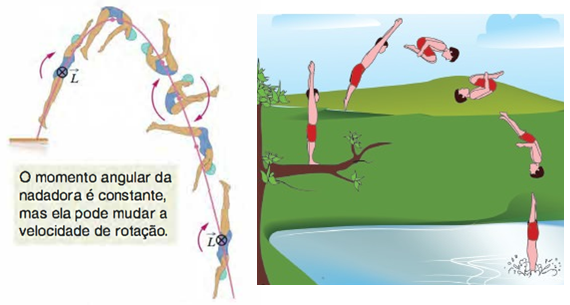
\includegraphics[scale=1.3]{images/i1.png}
  \caption{Saltos Ornamentais}
\end{figure}

O mesmo ocorre para os atletas da patinação no gelo. Como o torque exercido pelo piso de gelo no patinador é muito baixo – quase irrisório -, podemos considerar o momento angular praticamente constante, pois tratamos o sistema gelo + patinador como um sistema isolado. Dessa forma, quando ele recolhe os braços e pernas (aproximando-os do corpo), diminui consideravelmente seu momento de inércia, fazendo com que sua velocidade angular aumente e ele passa a girar com maior rapidez.\\ 

\begin{figure}[H]
  \centering
  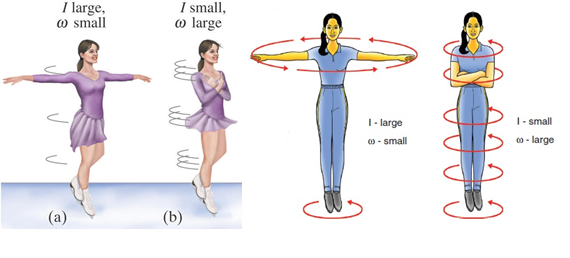
\includegraphics[scale=1.3]{images/i2.png}
  \caption{Patinação no Gelo}
\end{figure}

Analogamente, os ginastas das barras fixas utilizam a conservação do momento angular para realizarem seus movimentos de giro, ganhando ou perdendo velocidade conforme abrem ou fecham os braços e as pernas. \\

\begin{figure}[H]
  \centering
  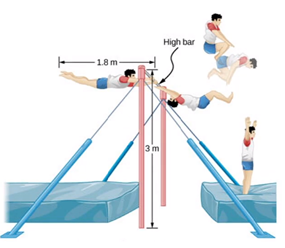
\includegraphics[scale=1.7]{images/i3.png}
  \caption{Ginástica - Barra Fixa }
\end{figure}

Então, mostramos a importância da lei de conservação do momento angular, que aplicada em sistemas isolados (ou quase isolados) nos fornece saltos e movimentos majestosos. Porém, em alguns casos essa conservação é motivo de alerta para nós.\\

Um exemplo desse, muito comum em veículos de manobras que realizam saltos, como motos e carros \textit{off-road}, pode ser observado nas competições de Mini Baja. Quando o carro salta de uma rampa e está no ar, não há torques externos agindo nele, então consideramos seu momento angular praticamente constante. Dessa maneira, a rotação das rodas é a responsável pela velocidade angular desse sistema, portanto, se frearmos diminuímos essa velocidade, e o carro como um todo tende a rotacionar no mesmo sentido das rodas (para frente), para compensar a falta de giro das rodas – por conta da conservação de momento-, fazendo com que o carro capote se frearmos com ele no ar. 
Caso realizemos o contrário, acelerando o carro com ele no ar, o chassi como um todo irá rodar no sentido oposto do aumento de velocidade das rodas (para trás) para compensar essa velocidade angular “positiva” nas rodas, mantendo constante o momento angular do sistema.\\ 

\textbf{b) Explique a demonstração do momento de inércia variável (banquinho giratório) apresentado na vídeo-aula.}\\

Ao estudarmos o assunto da conservação do momento angular, alguns exemplos clássicos são apresentados aos alunos. Um dos mais famosos, que tem fácil execução e pode ser feito até em sala de aula, é o experimento do “Banquinho Giratório”. Nesse exemplo, um banco – com pouco ou quase nenhum atrito – gira livremente em torno de um eixo vertical. Com a ajuda de rolamentos, que minimizam a força de atrito, podemos considerar o sistema banco + aluno como um sistema isolado, sem torques externos.\\

O estudante senta no banco e é posto em rotação com uma pequena velocidade angular inicial $\omega _1$, segurando dois halteres com os braços abertos. O vetor momento angular inicial L do aluno aponta para cima e está no mesmo eixo da rotação do banco. O estudante leva os halteres para próximo do peito, diminuindo o momento de inércia do valor inicial I$_1$ para um valor menor I$_2$ pois a massa dos halteres se aproxima do eixo de rotação. A velocidade angular do estudante aumenta consideravelmente, de $\omega _1$ para $\omega _2$, para poder compensar a diminuição do momento de inércia, conservando o momento angular. O estudante pode reduzir sua velocidade angular abrindo os braços novamente, afastando os halteres do eixo de rotação. Como já ressaltado, nenhum torque externo resultante age sobre o sistema formado pelo estudante, o banco e os halteres. Assim, o momento angular do sistema em relação ao eixo de rotação permanece constante, não importando como o estudante segura os halteres.

\begin{figure}[H]
  \centering
  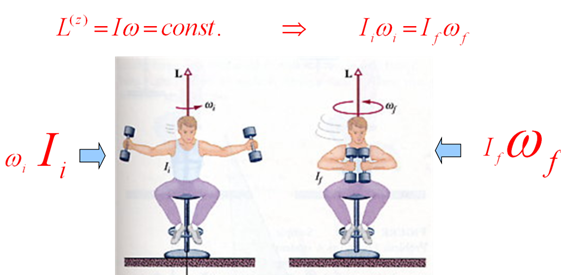
\includegraphics[scale=1.3]{images/i4.png}
  \caption{Banco Giratório}
\end{figure}

\textbf{c) Na vídeo-aula é apresentado a famosa demonstração do banquinho giratório com a roda de bicicleta. Explique o que acontece. Nas duas situações apresentadas como A e B indique o sentido de rotação da roda de bicicleta, justificando a sua resposta.}\\

Ainda podemos ressaltar um último experimento muito interessante que é o caso do banquinho giratório com a roda de bicicleta. Semelhantemente ao experimento anterior, um aluno senta em um banco, que gira sem atrito - não existindo torques externos sobre o sistema estudante-banco-roda, sendo considerado isolado. O aluno segura uma roda de bicicleta e no começo do experimento tanto o banco quanto a roda estão em repouso.\\

Em um certo momento a roda de bicicleta – que se encontra na horizontal – é posta para girar, criando um momento angular de rotação da roda, vertical. Quando o aluno levanta a roda, cria-se uma componente do momento angular ao longo do eixo z (para cima). Como o sistema é isolado, o momento angular deve ser conservado, então o banco começa a girar no sentido oposto da rotação da roda, de modo a criar um momento angular contrário ao criado pela roda.\\

Nesse experimento fica clara a conservação de momento angular na direção z (eixo para cima), pois inicialmente não havia momento nesse eixo. Ao inclinar a roda, surge uma componente de momento nesse eixo, no mesmo sentido da rotação imposta à roda de bicicleta. Mais que depressa, o banquinho começa a rodar no sentido oposto, para compensar a rotação que surge, buscando conservar o momento naquele eixo (que era nulo no início). No experimento do vídeo, não sabemos qual o sentido inicial de rotação da roda de bicicleta (que está coberta por um tampão), e são dadas duas situações:

\begin{itemize}
    \item Ao levantar a roda, o banco gira no sentido HORÁRIO.
    \item Ao levantar a roda, o banco gira no sentido ANTI-HORÁRIO.
\end{itemize}

Desse modo, como já discutimos acima, quando surge a componente do momento no eixo z, o banco gira no sentido oposto da roda para compensar essa rotação, então:

\begin{figure}[H]
  \centering
  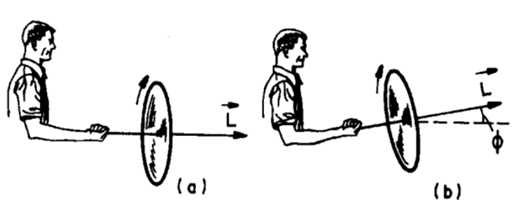
\includegraphics[scale=1.4]{images/i5.png}
  \caption{Roda de Bicicleta Giratória}
\end{figure}

\begin{figure}[H]
  \centering
  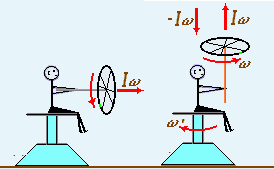
\includegraphics[scale=1.7]{images/i6.png}
  \caption{Banco Giratório com Roda de Bicicleta}
\end{figure}

\begin{itemize}
    \item Como o banco gira no sentido HORÁRIO, a roda inicialmente foi posta para girar no sentido ANTI-HORÁRIO.
    \item Como o banco gira no sentido ANTI-HORÁRIO, a roda inicialmente foi posta para girar no sentido HORÁRIO.
\end{itemize}



% =============== EXPERIMENTO 4 ===================== %

\subsection{Precessão do Giroscópio}

Baseado no video disponibilizado para esse experimento os dados que temos disponíveis são os seguintes:

\begin{table}[H]
    \centering
    \begin{tabular}{ |p{5cm}||p{2cm}||p{2cm}||p{2cm}|  }
        \hline
        \textbf{O que foi medido} & \textbf{Valor} & \textbf{Incerteza} & \textbf{Unidade}\\
        \hline
        Meio eixo (D)                               & 0.0565    & $\pm$ 0.0001  & m\\
        Diâmetro do eixo (d\textsubscript{eixo})    & 0.0070    & $\pm$ 0.0001  & m\\
        Raio externo (R\textsubscript{1})           & 0.0702    & $\pm$ 0.0001  & m\\
        Raio interno (R\textsubscript{2})           & 0.0625    & $\pm$ 0.0001  & m\\
        Largura externa (l\textsubscript{1})        & 0.0203    & $\pm$ 0.0001  & m\\
        Largura interna (l\textsubscript{2})        & 0.0043    & $\pm$ 0.0001  & m\\
        Massa do conjunto (M)                       & 1.116     & $\pm$ 0.001   & kg\\
        Densidade do material ($\rho _{aco}$)       & 8000.0    & -             & $\frac{kg}{m^3}$\\
        \hline
    \end{tabular}
    \caption{Dados físicos do Giroscópio}
\end{table}

\begin{table}[H]
    \centering
    \begin{tabular}{ |p{5cm}||p{2cm}||p{2cm}||p{2cm}|  }
        \hline
        \textbf{O que foi medido} & \textbf{Valor} & \textbf{Incerteza} & \textbf{Unidade}\\
        \hline
        Tempo 1-1 (t\textsubscript{11})     & 0.072     & $\pm$ 0.001   & s\\
        Tempo 1-2 (t\textsubscript{12})     & 0.135     & $\pm$ 0.001   & s\\
        Tempo 1-3 (t\textsubscript{13})     & 0.194     & $\pm$ 0.001   & s\\
        Velocidade 1 ($\omega _1$)          & 271.2     & $\pm$ 0.1     & $\frac{rad}{s}$\\
        \hline
        Tempo 2-1 (t\textsubscript{21})     & 0.073     & $\pm$ 0.001   & s\\
        Tempo 2-2 (t\textsubscript{22})     & 0.138     & $\pm$ 0.001   & s\\
        Tempo 2-3 (t\textsubscript{23})     & 0.198     & $\pm$ 0.001   & s\\
        Velocidade 2 ($\omega _2$)          & 255.6     & $\pm$ 0.1     & $\frac{rad}{s}$\\
        \hline
        Tempo 3-1 (t\textsubscript{31})     & 0.076     & $\pm$ 0.001   & s\\
        Tempo 3-2 (t\textsubscript{32})     & 0.144     & $\pm$ 0.001   & s\\
        Tempo 3-3 (t\textsubscript{33})     & 0.206     & $\pm$ 0.001   & s\\
        Velocidade 3 ($\omega _3$)          & 308.2     & $\pm$ 0.1     & $\frac{rad}{s}$\\
        \hline
        Tempo 4-1 (t\textsubscript{41})     & 0.074     & $\pm$ 0.001   & s\\
        Tempo 4-2 (t\textsubscript{42})     & 0.142     & $\pm$ 0.001   & s\\
        Tempo 4-3 (t\textsubscript{43})     & 0.205     & $\pm$ 0.001   & s\\
        Velocidade 4 ($\omega _4$)          & 256.4     & $\pm$ 0.1     & $\frac{rad}{s}$\\
        \hline
    \end{tabular}
    \caption{Dados experimentais do Giroscópio}
\end{table}

- Estimar a massa do giroscópio\\
- Calcular o momento de inercia dele\\
- Frequência estimada (4x) \\
\\
- Frequência real (4x)\\
- Determinar diretamente (pelo tempo) a frequência de precessão\\
- Comparar as frequências
